%%%%%%%%%%%%%%%%%%%%% PACKAGE IMPORTS %%%%%%%%%%%%%%%%%%%%%
\documentclass{article}
\usepackage{import}

\usepackage{amsmath, amsfonts, amsthm, amssymb}
\usepackage{lmodern}
\usepackage{microtype}
\usepackage{fullpage}       
\usepackage{changepage}
\usepackage{hyperref}
\usepackage{blindtext}
\hypersetup{
    colorlinks=true,
    linkcolor=blue,
    filecolor=magenta,      
    urlcolor=blue,
    pdftitle={Overleaf Example},
    pdfpagemode=FullScreen,
    }
\urlstyle{same}

\newenvironment{level}%
{\addtolength{\itemindent}{2em}}%
{\addtolength{\itemindent}{-2em}}

\usepackage{amsmath,amsthm,amssymb}

\usepackage[nooldvoltagedirection]{circuitikz}
\usetikzlibrary{decorations,arrows,shapes}

\usepackage{datetime}
\usepackage{etoolbox}
\usepackage{enumerate}
\usepackage{enumitem}
\usepackage{listings}
\usepackage{array}
\usepackage{varwidth}
\usepackage{tcolorbox}
\usepackage{amsmath}
\usepackage{circuitikz}
\usepackage{verbatim}
\usepackage[linguistics]{forest}
\usepackage{listings}
\usepackage{xcolor}
\renewcommand{\rmdefault}{cmss}


\newcommand\doubleplus{+\kern-1.3ex+\kern0.8ex}
\newcommand\mdoubleplus{\ensuremath{\mathbin{+\mkern-10mu+}}}

\definecolor{codegreen}{rgb}{0,0.6,0}
\definecolor{codegray}{rgb}{0.5,0.5,0.5}
\definecolor{codepurple}{rgb}{0.58,0,0.82}
\definecolor{backcolour}{rgb}{0.95,0.95,0.92}

\lstdefinestyle{mystyle}{
    language=Python,
    basicstyle=\ttfamily\small,
    keywordstyle=\color{blue},
    stringstyle=\color{red},
    commentstyle=\color{green},
    morecomment=[l][\color{magenta}]{\#},
    backgroundcolor=\color{backcolour},   
    breakatwhitespace=false,         
    breaklines=true,                 
    captionpos=b,                    
    keepspaces=true,                 
    numbers=left,                    
    numbersep=5pt,                  
    showspaces=false,                
    showstringspaces=false,
    showtabs=false,                  
    tabsize=2
}

\lstset{style=mystyle}
\setlength{\parindent}{0pt}
\setlength{\parskip}{5pt plus 1pt}

\providetoggle{questionnumbers}
\settoggle{questionnumbers}{true}
\newcommand{\noquestionnumbers}{
    \settoggle{questionnumbers}{false}
}

\newcounter{questionCounter}
\newenvironment{question}[2][\arabic{questionCounter}]{%
    \ifnum\value{questionCounter}=0 \else {\newpage}\fi%
    \setcounter{partCounter}{0}%
    \vspace{.25in} \hrule \vspace{0.5em}%
    \noindent{\bf \iftoggle{questionnumbers}{Question #1: }{}#2}%
    \addtocounter{questionCounter}{1}%
    \vspace{0.8em} \hrule \vspace{.10in}%
}

\newcounter{partCounter}[questionCounter]
\renewenvironment{part}[1][\alph{partCounter}]{%
    \addtocounter{partCounter}{1}%
    \vspace{.10in}%
    \begin{indented}%
       {\bf (#1)} %
}{\end{indented}}

\def\indented#1{\list{}{}\item[]}
\let\indented=\endlist
\def\show#1{\ifdefempty{#1}{}{#1\\}}
\def\IMP{\longrightarrow}
\def\AND{\wedge}
\def\OR{\vee}
\def\BI{\leftrightarrow}
\def\DIFF{\setminus}
\def\SUB{\subseteq}


\newcolumntype{C}{>{\centering\arraybackslash}m{1.5cm}}
\renewcommand\qedsymbol{$\blacksquare$}
\newtcolorbox{answer}
{
  colback   = green!5!white,    % Background colorucyitc,
  colframe  = green!75!black,   % Outline color
  box align = center,           % Align box on text line
  varwidth upper,               % Enables multi line input
  hbox                          % Bounds box to text width
}

\newcommand{\myhwname}{CSE 447 Assignment 2}
\newcommand{\myname}{Sebastian Liu}
\newcommand{\myemail}{ll57@cs.washington.edu}
\newcommand{\mysection}{AB}
\newcommand{\dollararrow}{\stackrel{\$}{\leftarrow}}
%%%%%%%%%%%%%%%%%%%%%%%%%%%%%%%%%%%%%%%%%%%%%%%%%%%%%%%%%%%

%%%%%%%%%%%%%%%%%%% Document Options %%%%%%%%%%%%%%%%%%%%%%
\noquestionnumbers
%%%%%%%%%%%%%%%%%%%%%%%%%%%%%%%%%%%%%%%%%%%%%%%%%%%%%%%%%%%

%%%%%%%%%%%%%%%%%%%%%%%% WORK BELOW %%%%%%%%%%%%%%%%%%%%%%%%
\begin{document}

\begin{center}
    \textbf{Assignment 2} \bigskip
\end{center}

%%%%%%%%%%%%%%%%%%%%%%%% Task 1 %%%%%%%%%%%%%%%%%%%%%%%%M
\begin{question}{Understanding Attentions (20\%)}
    \setcounter{section}{1}
    \setcounter{subsection}{1}
    \subsection{Selection via Attention}
    \begin{part}[1.2.1]
       \begin{answer}
        Assume $q = \begin{bmatrix}
            x_0 & x_1 & x_2
        \end{bmatrix}$ and we have large scalar $S = 1e5$.\\
        We have $A = qK^\top = \begin{bmatrix}
            x_0k_{0,0} + x_1k_{0,1} + x_2k_{0,2} \\
            x_0k_{1,0} + x_1k_{1,1} + x_2k_{1,2} \\
            x_0k_{2,0} + x_1k_{2,1} + x_2k_{2,2} \\
            x_0k_{3,0} + x_1k_{3,1} + x_2k_{3,2} \\
        \end{bmatrix}^\top$,\\
        $A' = \text{softmax}(A) = \begin{bmatrix}
            \frac{\exp( x_0k_{0,0} + x_1k_{0,1} + x_2k_{0,2})}{\sum_{j=0}^{3} \exp(x_0k_{j,0} + x_1k_{j,1} + x_2k_{j,2})} \\
            \frac{\exp(x_0k_{1,0} + x_1k_{1,1} + x_2k_{1,2})}{\sum_{j=0}^{3} \exp(x_0k_{j,0} + x_1k_{j,1} + x_2k_{j,2})} \\
            \frac{\exp(x_0k_{2,0} + x_1k_{2,1} + x_2k_{2,2})}{\sum_{j=0}^{3} \exp(x_0k_{j,0} + x_1k_{j,1} + x_2k_{j,2})} \\
            \frac{\exp(x_0k_{3,0} + x_1k_{3,1} + x_2k_{3,2})}{\sum_{j=0}^{3} \exp(x_0k_{j,0} + x_1k_{j,1} + x_2k_{j,2})} \\
        \end{bmatrix}^\top$, \\
        and finally $O = A' V = \\ \begin{bmatrix}
            \frac{\exp(x_0k_{0,0} + x_1k_{0,1} + x_2k_{0,2})}{\sum_{j=0}^{3} \exp(x_0k_{j,0} + x_1k_{j,1} + x_2k_{j,2})} v_{0,0} + 
            \frac{\exp(x_0k_{1,0} + x_1k_{1,1} + x_2k_{1,2})}{\sum_{j=0}^{3} \exp(x_0k_{j,0} + x_1k_{j,1} + x_2k_{j,2})} v_{1,0} \\+
            \frac{\exp(x_0k_{2,0} + x_1k_{2,1} + x_2k_{2,2})}{\sum_{j=0}^{3} \exp(x_0k_{j,0} + x_1k_{j,1} + x_2k_{j,2})} v_{2,0} +
            \frac{\exp(x_0k_{3,0} + x_1k_{3,1} + x_2k_{3,2})}{\sum_{j=0}^{3} \exp(x_0k_{j,0} + x_1k_{j,1} + x_2k_{j,2})} v_{3,0} \\\\
            \frac{\exp(x_0k_{0,0} + x_1k_{0,1} + x_2k_{0,2})}{\sum_{j=0}^{3} \exp(x_0k_{j,0} + x_1k_{j,1} + x_2k_{j,2})} v_{0,1} +
            \frac{\exp(x_0k_{1,0} + x_1k_{1,1} + x_2k_{1,2})}{\sum_{j=0}^{3} \exp(x_0k_{j,0} + x_1k_{j,1} + x_2k_{j,2})} v_{1,1} \\+
            \frac{\exp(x_0k_{2,0} + x_1k_{2,1} + x_2k_{2,2})}{\sum_{j=0}^{3} \exp(x_0k_{j,0} + x_1k_{j,1} + x_2k_{j,2})} v_{2,1} +
            \frac{\exp(x_0k_{3,0} + x_1k_{3,1} + x_2k_{3,2})}{\sum_{j=0}^{3} \exp(x_0k_{j,0} + x_1k_{j,1} + x_2k_{j,2})} v_{3,1} \\\\
            \frac{\exp(x_0k_{0,0} + x_1k_{0,1} + x_2k_{0,2})}{\sum_{j=0}^{3} \exp(x_0k_{j,0} + x_1k_{j,1} + x_2k_{j,2})} v_{0,2} +
            \frac{\exp(x_0k_{1,0} + x_1k_{1,1} + x_2k_{1,2})}{\sum_{j=0}^{3} \exp(x_0k_{j,0} + x_1k_{j,1} + x_2k_{j,2})} v_{1,2} \\+
            \frac{\exp(x_0k_{2,0} + x_1k_{2,1} + x_2k_{2,2})}{\sum_{j=0}^{3} \exp(x_0k_{j,0} + x_1k_{j,1} + x_2k_{j,2})} v_{2,2} +
            \frac{\exp(x_0k_{3,0} + x_1k_{3,1} + x_2k_{3,2})}{\sum_{j=0}^{3} \exp(x_0k_{j,0} + x_1k_{j,1} + x_2k_{j,2})} v_{3,2} 
 
        \end{bmatrix}^\top$\\\\
        We can see that to get $O = \begin{bmatrix}
            v_{0,0} & v_{0,1} & v_{0,2} \\
        \end{bmatrix}$, we need the first term of $A'$ ($\frac{\exp( x_0k_{0,0} + x_1k_{0,1} + x_2k_{0,2})}{\sum_{j=0}^{3} \exp(x_0k_{j,0} + x_1k_{j,1} + x_2k_{j,2})}$) to be
        significanly larger than the other terms, so the results of $\frac{\exp(x_0k_{0,0} + x_1k_{0,1} + x_2k_{0,2})}{\sum_{j=0}^{3} \exp(x_0k_{j,0} + x_1k_{j,1} + x_2k_{j,2})} v_{0,i}$
        dominate the sum in $O$. \\
        Thus, $\exp(x_0k_{0,0} + x_1k_{0,1} + x_2k_{0,2})$ needs to be significantly larger than the other terms in $A$, to achieve this we need a $q$ that
        scales the first term of $A$ to be larger than the other terms. This means that $q$ needs to be a vector that align with $k_0$ and
        has a large magnitude, then the exponential function will do the amplification. \\
        Therefore, the query vector should be $\boxed{q = S \cdot k_0 = \begin{bmatrix}
            S \cdot k_{0,0} & S \cdot k_{0,1} & S \cdot k_{0,2}
        \end{bmatrix} = \begin{bmatrix}
            0.47S & 0.65S & 0.60S
        \end{bmatrix}}$. By setting a query vector to a specific scaled key vector, we are essentially focusing the model's attention to the corresponding value vectors.

        \end{answer}
    \end{part}
\newpage
    \begin{part}[1.2.2]
        \begin{answer}
            Similar idea to 1.2.1, but instead of the first element of $A'$ dominating the sum in $O$, we want the diagonal elements of $A'$ to dominate the sum of each row
            of $O$. From 1.2.1, we know that we can achieve this by scaling each key vector by a large scalar to focus the model's attention to each of the value vectors. \\
            Therefore, we have:\\ $\boxed{Q = S \cdot K = \begin{bmatrix}
                S \cdot k_0 \\
                S \cdot k_1 \\
                S \cdot k_2 \\
                S \cdot k_3 \\
            \end{bmatrix} = \begin{bmatrix}
                S \cdot k_{0,0} & S \cdot k_{0,1} & S \cdot k_{0,2} \\
                S \cdot k_{1,0} & S \cdot k_{1,1} & S \cdot k_{1,2} \\
                S \cdot k_{2,0} & S \cdot k_{2,1} & S \cdot k_{2,2} \\
                S \cdot k_{3,0} & S \cdot k_{3,1} & S \cdot k_{3,2} \\
            \end{bmatrix} = \begin{bmatrix}
                \phantom{-}0.47S &  \phantom{-}0.65S &  \phantom{-}0.60S \\
                \phantom{-}0.64S &  \phantom{-}0.50S & -0.59S \\
                -0.03S & -0.48S & -0.88S \\
                \phantom{-}0.43S & -0.83S &  \phantom{-}0.35S \\
            \end{bmatrix}}$
        \end{answer}
     \end{part}

     \begin{part}[1.2.3]
        \begin{answer}
            It allows language models to highlight the important parts of a sequence, so the model can directly reference specific details from the input into the output, 
            which might improve accuracy, and appropriateness in certain contexts. It might also give better continuity in longer outputs.
         \end{answer}
     \end{part}
\end{question}

\subsection{Averaging via Attention}
\begin{part}[1.3.1]
    \begin{answer}
        Referring to the calculation in 1.2.1, we can see that if we want to average all the value vectors, we need each element of $A'$ to be
        roughly equal. This means we need $x_0k_{0,0} + x_1k_{0,1} + x_2k_{0,2}$ to be roughly equal to $x_0k_{1,0} + x_1k_{1,1} + x_2k_{1,2}$ and so on. \\
        We see a simple way to achieve this is to set each element in $q$ to be the mean of each corresponding column in $K$ and we can also scale it down to further
        to reduce the variance. So we can have $\mu_{k_{,0}}k_{0,0} + \mu_{k_{,1}}k_{0,1} + \mu_{k_{,2}}k_{0,2}$ be roughly equal
        to $\mu_{k_{,0}}k_{1,0} + \mu_{k_{,1}}k_{1,1} + \mu_{k_{,2}}k_{1,2}$ and so on.\\

        Therefore, we have:\\ $\boxed{q = \frac{k_1 + k_2 + k_3 + k_4}{4} = \begin{bmatrix}
            \frac{0.47 + 0.64 - 0.03 + 0.43}{4} & \frac{0.65 + 0.50 - 0.48 - 0.83}{4} & \frac{0.60 - 0.59 - 0.88 + 0.35}{4}
        \end{bmatrix}}$. \\
    \end{answer}
 \end{part}

 \begin{part}[1.3.2]
    \begin{answer}
        Similar to 1.3.1, but instead of taking the mean of columns of all rows (key vectors) in $K$, we only take the mean of the first two rows (key vectors) in $K$.
        Depending on the result, we could scale up the query vector to slightly  increase the attention on the first two value vectors. \\
        Therefore, we have:\\ $\boxed{q = \frac{k_1 + k_2}{2} = \begin{bmatrix}
            \frac{0.47 + 0.64}{2} & \frac{0.65 + 0.50}{2} & \frac{0.60 - 0.59}{2}
        \end{bmatrix}}$. \\
     \end{answer}
 \end{part}
\newpage
 \begin{part}[1.3.3]
    \begin{answer}
        It gives the model ability to condense different information from a sequence, which allows the model to
        better capture main ideas of a text. It might be good for summarization tasks.
     \end{answer}
 \end{part}

%%%%%%%%%%%%%%%%%%%%%%%% Task 2 %%%%%%%%%%%%%%%%%%%%%%%%
\begin{question}{2 Building Your Own Mini Transformer (40\%)}
    \setcounter{section}{2}
    \setcounter{subsection}{1}
    \subsection{Experiment with Your Implementation of Attention}
    \subsubsection{Experiment 1: Dot-Product Attention v.s. Additive Attention}
    \begin{part}[2.2.1.1 Setup]
        \begin{answer}
            Attention mechanisms allow models to dynamically focus on different parts of the input data when producing an output.
            This experiment compares two attention mechanisms, dot-product attention and additive attention,
            and try to understand how different attention mechanisms affect the performance in the context of a mini-GPT model. \\\\
            Both models has the same architecture except for how they compute the attention scores:\\\\
            \textbf{Dot-product attention} computes the attention scores based on the dot product of query and key vectors and then scaled down with a scale factor. Assume
            we have query matrix $Q$, key matrix $K$, embedding dimensionality $n_{embd}$, and number of heads $n_{head}$, then the attention score matrix $A_{\text{dot-product}}$, is computed as follows:
            $$A_{\text{dot-product}} = \frac{QK^\top}{\sqrt{n_{embd}/n_{head}}}$$

            \textbf{Additive attention} computes attention scores by adding the query and key vectors followed by a nonlinear tanh transformation. Here, the attention score matrix $A$ is computed as follows:
            $$A_{\text{additive}} = W_2 (\tanh(W_1([Q;K])))$$ where $W_1$ and $W_2$ are learned weight matrices. \\\\

            Both models are trained on the same dataset which has the following properties:
            \begin{itemize}
                \item total training tokens: 1,561,375
                \item \# of unique tokens: 80,663
                \item sequence length (in tokens) distribution :\\
                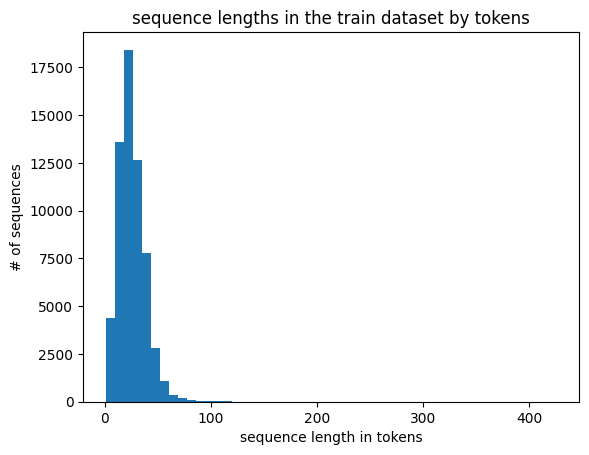
\includegraphics[width=0.44\linewidth]{sequence_length_in_the_train_dataset_by_tokens.png}
            \end{itemize}

         \end{answer}
     \end{part}
     \begin{part}[2.2.1.1 contd.]
        \begin{answer}
            Since a majority of tokens are below 100 tokens, we truncate to 100 tokens for performance reasons.
            Both models has 1.41 million parameters, and are trained for 1 epoch with a batch size of 32. The learning rate is set to 5e-4.\\\\
            My hypothesis is that dot-product attention will compute faster given its simplicity, while additive attention may
            give a slight improvement performance, since its nonlinearity gives it the ability to model more complex relationships.
        \end{answer}
     \end{part}

     \begin{part}[2.2.1.2 Results]
        \begin{answer}
                Table 1: Training Time and Loss Comparison\\
            \begin{tabular}{|c|c|c|}
                \hline
                \textbf{} & \textbf{Dot-Product} & \textbf{Additive Attention} \\
                \hline
                \textbf{Training Time} &  3:35 &  20:29 \\
                \hline
                \textbf{Final Training Loss} &  5.85 &  5.72\\
                \hline
                \textbf{Traing Step vs. Loss} & 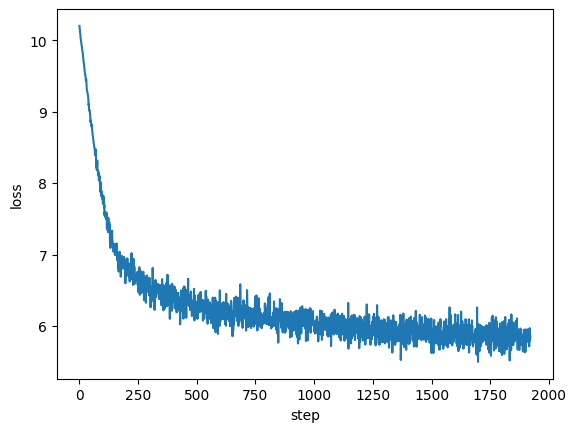
\includegraphics[width=0.3\linewidth]{../experiments/wo_changes/training_step_vs_loss.png} &  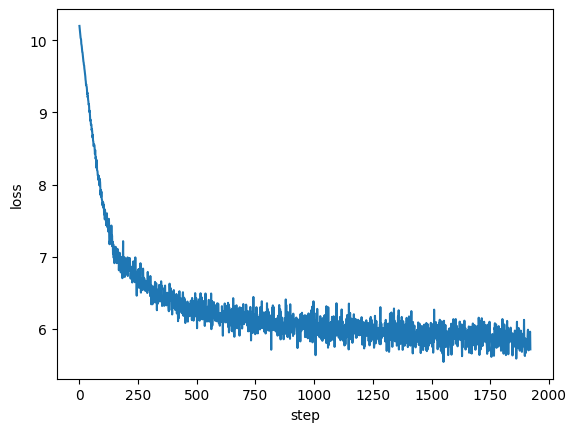
\includegraphics[width=0.3\linewidth]{../experiments/additive_attention/training_step_vs_loss.png}\\
                \hline
            \end{tabular}\\\\
            
            Table 2: Testing Loss Comparison\\
            \#1: "After learning language models model natural language."\\
            \#2: "The quick brown fox jumps over the lazy dog."\\
            \#3: "Amidst the twilight, the ancient ruins whispered secrets long forgotten."\\
            \#4: "Quantum entanglement fascinates physicists and philosophers alike, bridging worlds with invisible threads."\\
            \begin{tabular}{|c|c|c|}
                \hline
                \textbf{} & \textbf{Dot-Product} & \textbf{Additive Attention} \\
                \hline
                \textbf{Sentence\#1} & 9.459  & 9.114  \\
                \hline
                \textbf{Sentence\#2} & 6.742  & 6.478  \\
                \hline
                \textbf{Sentence\#3} & 8.199  & 7.895  \\
                \hline
                \textbf{Sentence\#4} & 6.355  & 6.327 \\
                \hline
            \end{tabular}\\\\

            Table 3: Perplexity Comparison\\
            \begin{tabular}{|c|c|c|}
                \hline
                \textbf{} & \textbf{Dot-Product} & \textbf{Additive Attention} \\
                \hline
                \textbf{Sentence\#1} & 12820.091  &  9083.743 \\
                \hline
                \textbf{Sentence\#2} &  847.358 &  650.523 \\
                \hline
                \textbf{Sentence\#3} &  3636.979 &  2684.190 \\
                \hline
                \textbf{Sentence\#4} &  575.407 &  559.330 \\
                \hline
                \textbf{Train Perplexity} &  401.043 &  405.255 \\
                \hline
                \textbf{Dev Perplexity} &  380.805 &  385.998 \\
                \hline
            \end{tabular}
         \end{answer}
     \end{part}
\newpage
\begin{part}[2.2.1.2 contd.]
    \begin{answer}
        Sample Outputs Comparison:\\
        \textbf{Dot-Product Attention:}
        \begin{enumerate}
            \item $<$START$>$ A age on evidence care nothing , United States are up the people , which is by the attacks for a barrel to big spending on this media when confirm the pledged , Price , low sea after the bring her Life , but she works in Steven Sox media , however . became a presence and then them attempt in December with an discovered of West organization days said , 2009 . $<$STOP$>$
            \item $<$START$>$ And over the House will keep Gordon tour by the department of all its being Big taxable many months were $<$UNK$>$ , on its Radio feed in the new building . $<$STOP$>$
            \item $<$START$>$ dramatic Ireland cents in the New candidates which could take the owners previously sent much been linked to $<$UNK$>$ , rise . $<$STOP$>$
            \item $<$START$>$ A eyes of photos is explained the riding , with their negligence stripped of Afghan 2008 program of 2008 . $<$STOP$>$
            \item $<$START$>$ After Somali government of print broke out the final two documentary Alinghi and $<$UNK$>$ - 4-3 oil will be child and strikes in Wednesday . $<$STOP$>$
        \end{enumerate}
        \textbf{Additive Attention:}
        \begin{enumerate}
            \item $<$START$>$ " I were only that may should not the violence only much time for something president are at particles it 's proposal . $<$STOP$>$
            \item $<$START$>$ All of taking European band perceived $<$UNK$>$ $<$UNK$>$ , Antarctic and the third relatives as fans UCLA place , a profits were singer dangerous . $<$STOP$>$
            \item $<$START$>$ Anbar , received an threat of them on by out up by much parents , reaching out the church agent . $<$STOP$>$
            \item $<$START$>$ tunnels and earnings Bush soldiers are 20 points to reforms -- but today . $<$STOP$>$
            \item $<$START$>$ He is include estimates of your ; stuff managed to fix to answer scandal . $<$STOP$>$
        \end{enumerate}
    \end{answer}
\end{part}

     \begin{part}[2.2.1.3 Explantaion and Interpretation]
        \begin{answer}
            \textbf{Training Time and Loss:}
            Table 1 indicates that models using dot-product attention required significantly less training time (3:35) compared to additive attention (20:29).
            From the training step vs. loss plots, we can see that the loss of both models decreases around the same rate.
            However, additive attention achieved a slightly lower final training loss (5.72) compared to dot-product attention (5.85). This slight difference might
            not speak much about the performance of the models, but when changes the hyperparameters, the final loss stayed consistently lower for the additive attention model (data not shown here),
            which might suggest that the additive attention model is slightly better at capturing the relationships between the tokens in the training data. However, given the significant 
            increase in training time, the improvement in performance might not be worth the trade-off.
         \end{answer}
     \end{part}
\newpage
     \begin{part}[2.2.1.3 contd.]
        \begin{answer}
            \textbf{Testing Loss and Perplexity:}
            Table 2 and Table 3 present the loss and perplexity comparisons. Same story goes here, across four different sentences,
            additive attention consistently outperformed dot-product attention in terms of both lower testing loss and perplexity by a tiny margin.
            However, additive attention did have slightly higher training and dev perplexity (405.255 and 385.998) compared to dot-product attention (401.043 and 380.805),
            which might suggest that the model is overfitting the training data.
            In general, the differences in loss and perplexity are not significant enough to suggest that additive attention is significantly better than dot-product attention. \\\\

            \textbf{Sample Outputs:}
            Both models produced outputs that are mostly nonsensical, but one observation is that the outputs from dot-product attention are slightly more
            coherent than those from additive attention. Also, dot-product attention seems to produce longer sequences on average than additive attention.\\\\

            \textbf{Conclusion:}
            In the context of this experiment, dot-product attention is simpler, more efficient, and produces comparable results to additive attention.
            While additive attention demonstrates slightly superior performance in terms of loss and perplexity, it took significantly longer to train.
            In theory, additive attention should be able to model more complex relationships between tokens due to its nonlinearity, but the results of this experiment
            suggest that the performance improvement is not significant enough to justify the trade-off in training time.
            One possible explanation for the not so significant improvement in performance is that the training data used in this experiment
            might not be complex enough to fully leverage the modeling capabilities of additive attention. Given the restraint in computational resources and time in
            this experiment, dot-product attention is a more practical choice for the mini-GPT model.
            Future work could involve training the models on more complex datasets to see if additive attention can demonstrate more significant performance improvements.
        \end{answer}
     \end{part}
     \subsubsection{Experiment 2: Do We Need All Three of Q, K, and V?}
            \begin{answer}
                \textbf{Setup:}
                Similar to 2.2.1.1, we compare three models with the same architecture (both with dot-product attention) except for model 1
                has all three Q, K, and V used different projections, model 2 has only Q and K sharing the same projection, and model 3 has all three Q, K, and V sharing the same projection.\\\\
                \textbf{Results and Interpretation:}
                We failed to produce any results with any meaningful differences among the three models in terms of training time, loss, perplexity, and sample outputs.
                Even with tuning the hyperparameters (learning rate, batch size, training time, embedding dimensionality etc.),
                all three models produced almost identical results, which might suggest that in the context of this experiment, the model's performance is not sensitive to the
                different projection methods used for Q, K, and V. This might be due to the simplicity of the dataset used in this experiment, which might not require the model to
                fully leverage the different projection methods to capture the relationships between tokens.
             \end{answer}
      \newpage
         \subsubsection{Experiment 3: 0 Masking v.s. -Inf Masking}
        \begin{part}[2.2.3.1 Setup]
            \begin{answer}
                Similar to 2.2.1.1, we compare two models with the same architecture (both with dot-product attention) except for model 1
                used the naive masking approach of setting attention values to 0 after the softmax operation, and model 2 used the more standard approach
                of setting attention values to $-\infty$ before softmax.
             \end{answer}
         \end{part}
    
         \begin{part}[2.2.3.2 Results]
            \begin{answer}
                Table 1: Training Time and Loss Comparison\\
            \begin{tabular}{|c|c|c|}
                \hline
                \textbf{} & \textbf{$-\infty$ Masking} & \textbf{$0$ Masking} \\
                \hline
                \textbf{Training Time} &  3:35 &  2:32 \\
                \hline
                \textbf{Final Training Loss} &  5.85 &  5.27\\
                \hline
                \textbf{Traing Step vs. Loss} & 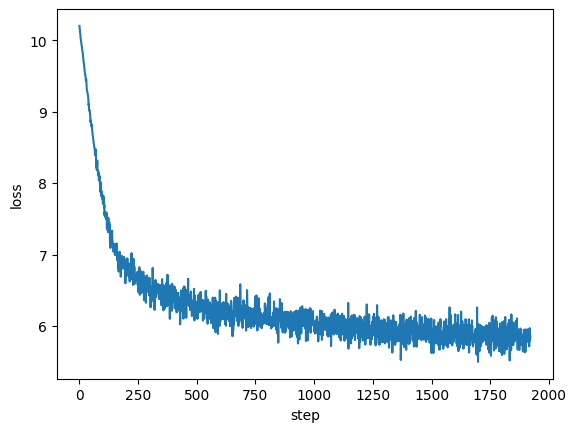
\includegraphics[width=0.3\linewidth]{../experiments/wo_changes/training_step_vs_loss.png} &  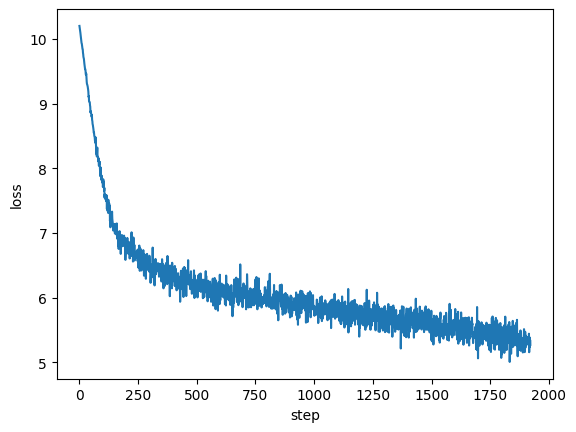
\includegraphics[width=0.3\linewidth]{../experiments/masking/training_step_vs_loss.png}\\
                \hline
            \end{tabular}\\\\
            
            Table 2: Testing Loss Comparison \;\;\;\;\;\;\;\;\;\;\;\;\;\;\;\;\;\;\;  Table 3: Perplexity Comparison\\
            \begin{tabular}{|c|c|c|}
                \hline
                \textbf{} & \textbf{$-\infty$ Masking} & \textbf{$0$ Masking} \\
                \hline
                \textbf{Sentence\#1} & 9.459  & 8.430  \\
                \hline
                \textbf{Sentence\#2} & 6.742  & 5.466  \\
                \hline
                \textbf{Sentence\#3} & 8.199  & 6.271  \\
                \hline
                \textbf{Sentence\#4} & 6.355  & 4.995 \\
                \hline
            \end{tabular}
            \begin{tabular}{|c|c|c|}
                \hline
                \textbf{} & \textbf{$-\infty$ Masking} & \textbf{$0$ Masking} \\
                \hline
                \textbf{Sentence\#1} & 12820.091  &  4584.009 \\
                \hline
                \textbf{Sentence\#2} &  847.358 &  236.421 \\
                \hline
                \textbf{Sentence\#3} &  3636.979 &  528.771 \\
                \hline
                \textbf{Sentence\#4} &  575.407 &  147.611 \\
                \hline
                \textbf{Train Perplexity} &  401.043 &  200.316 \\
                \hline
                \textbf{Dev Perplexity} &  380.805 &  186.542 \\
                \hline
            \end{tabular} \\\\\
            Sample Outputs Comparison:\\
        \textbf{$-\infty$ Masking:} (The same as dot-product attention outputs in 2.2.1.2)\\\\
        \textbf{0 Masking:}
        \begin{enumerate}
            \item $<$START$>$ $<$UNK$>$ . $<$STOP$>$
            \item $<$START$>$ And over " " " " $<$STOP$>$
            \item $<$START$>$ dramatic " " has by " " which could " $<$STOP$>$
            \item $<$START$>$ A " $<$STOP$>$
            \item $<$START$>$ After " " " " " said " I " " " " he I " " will I " " " " " " She 't " not " $<$STOP$>$
        \end{enumerate}
         \end{answer}
         \end{part}
\newpage
         \begin{part}[2.2.3.3 Explanation \& Interpretation]
            \begin{answer}
                \textbf{Training Time and performance:}
                By looking at Table 1, 2 and 3, it seems that the naive $0$ masking approach significantly outperformed the standard $-\infty$ masking approach in terms of both training time and performance.
                0 masking was nearly $30\% $ faster to train and achieved a lower final training loss (5.27) compared to $-\infty$ masking (5.85). 
                The training step vs. loss plots also show that the loss of the 0 masking model converged than the $-\infty$ masking model. The same goes for the testing loss and perplexity,
                where the 0 masking model consistently outperformed the $-\infty$ masking model across four different test sentences and in both training and dev perplexity by a large margin. \\
                Did we just found a new state-of-the-art masking approach? \\\\
                \textbf{Sample Outputs:}
                The answer is NO! The sample outputs from the 0 masking model barely produced any english words, it consist of mostly $<$UNK$>$ tokens and punctuation marks, which suggests that the model
                failed to learn anything meaningful from the training data. This is in stark contrast to the outputs from the $-\infty$ masking model, which although nonsensical, at least contained some meaningful english sequences.\\\\
                \textbf{Interpretation and Conclusion:}
                The results of this experiment suggest that the naive $0$ masking approach does not work for training transformer models. The reason for the "significant improvement" in performance
                is likely due to the zeroing out of the attention scores, which effectively allowed the model to cheat during the test and prevented it from learning anything meaningful from the training data.
            \end{answer}
         \end{part}
\end{question}

%%%%%%%%%%%%%%%%%%%%%%%% Task 3 %%%%%%%%%%%%%%%%%%%%%%%%
\begin{question}{3 HuggingFace (40\%) }
    \setcounter{section}{3}
    \setcounter{subsection}{1}
    \subsection{Finetunning Your Own RoBERTa Model}
    \begin{part}[Q1.1]
        \begin{answer}

        \end{answer}
    \end{part}

    \begin{part}[Q1.2]
        \begin{answer}

        \end{answer}
    \end{part}

    \begin{part}[Q2.1]
        \begin{answer}

        \end{answer}
    \end{part}

    \begin{part}[Q2.2]
        \begin{answer}

        \end{answer}
    \end{part}

    \begin{part}[Q2.3]
        \begin{answer}

        \end{answer}
    \end{part}

    \begin{part}[Q3.1]
        \begin{answer}

        \end{answer}
    \end{part}

    \begin{part}[Q3.2]
        \begin{answer}

        \end{answer}
    \end{part}

    \begin{part}[Q3.3]
        \begin{answer}

        \end{answer}
    \end{part}

    \begin{part}[Q4.1]
        \begin{answer}

        \end{answer}
    \end{part}

    \begin{part}[Q4.2]
        \begin{answer}

        \end{answer}
    \end{part}

    \begin{part}[Q4.3]
        \begin{answer}

        \end{answer}
    \end{part}

    \begin{part}[Q4.4]
        \begin{answer}

        \end{answer}
    \end{part}

    \begin{part}[Q4.5]
        \begin{answer}

        \end{answer}
    \end{part}

    \begin{part}[Q4.6]
        \begin{answer}

        \end{answer}
    \end{part}

    \begin{part}[Q4.7]
        \begin{answer}

        \end{answer}
    \end{part}

    \begin{part}[Q5.1]
        \begin{answer}

        \end{answer}
    \end{part}
\end{question}
\end{document}

